\chapter{Überblick über Modern OpenGL}
\label{chap:modern-opengl}

Mit der Abkehr von der Fixed-Function Pipeline (oder kurz Fixed Pipeline) begann die Ära von \textit{Modern OpenGL}. Seit dem ist es möglich mit eigenen Shader-Programmen, in \textit{OpenGL} meist geschrieben in der Sprache GLSL, die einzelnen Stufen der Renderpipline anzupassen. Zusätzlich wurden in \textit{OpenGL} Kontext Profile eingeführt, die es ermöglichen, Abschnitte der Spezifikation als ungültig bzw. \textit{deprecated} zu deklaieren. Das Profil wird bei der Erzeugung eines \textit{OpenGL} Kontextes angegeben. Hierbei wird zwischen folgenden Profilen unterschieden:

\begin{enumerate}[leftmargin=3.5cm]
\item[\textit{Core}] \hfill \\
	Spiegelt den aktuellen Stand der \ac{API} wieder. Alle, in vergangenen Versionen als \textit{deprecated} markierten Abschnitte, sind entfernt.
\item[\textit{Compatibility}] \hfill \\
	Stellt die komplette \ac{API} zur Verfügung, inklusive der als \textit{deprecated} markierten Abschnitte. 
\item[\textit{Forward-Compatible}] \hfill \\
	Alle, in der aktuellen Version für zukünftige Versionen als \textit{deprecated} markierten Abschnitte, sind entfernt.
\end{enumerate}

\section{Von Fixed Pipeline zu Shadern}

\begin{wrapfigure}{r}{0.4\linewidth}
\begin{centering}
	
\includegraphics[width=.5\textwidth]{OpenGL_Nov14}
\end{centering}
\end{wrapfigure}

Die Abkehr von der Fixed Pipeline erlaubte völlig neue Konzepte im Echtzeit-Rendering, anfangen von eigenen, anstatt fest vorgegeben, Beleuchtungsmodellen (siehe \fref{chap:pbr}) hin zu ausschließlich Fragment Shader basierten Grafikdemos\footnote{https://www.shadertoy.com/view/Xtf3Rn} sowie neuen Echzeit-Rendering Konzepten\footnote{http://iquilezles.org/www/articles/raymarchingdf/raymarchingdf.htm}.

Während ursprünglich der Szene-Graph fest von OpenGL vorgegeben war und Vertices mindestens einmal jeweils \textbf{einzeln}\footnote{ zum Beispiel mit \texttt{glVertex4f}} von der CPU auf die GPU geladen werden mussten, wurde das mit der Abkehr von der Fixed-Function Pipeline geändert. Buffer Objekte wurden immer wichtiger.

Mit Vertex Buffern können Vertices nun im Block auf die Grafikkarte geladen werden. Das führt unter anderem dazu, dass der Overhead, Vertices zur Grafikkarte zu schicken, sich deutlich reduzierte. Zum anderen erlauben Vertex-Shader die flexiblere Transformation der Vertices auf der Grafikkarte. Mittlerweile gibt es weitere unterschiedliche Buffer Typen für unterschiedliche Zwecke. Beispielsweise generische Shader Storage Buffer, die von allen Shader-Stufen gelesen und geschrieben werden können. Dies erlaubt Verfahren, die vorher ausschließlich auf der CPU ausgeführt werden konnten, komplett auf die Grafikkarte auszulagern, beispielsweise das View-Frustum Culling \parencite{Barczak2008}. Mit dem \textit{Unified Shader Model}, ein einheitlicher Befehlssatz für alle Shader Stufen, ist es zudem möglich, dass die Recheneinheiten der Grafikkarte entsprechend der Auslastung den jeweiligen Shader Stufen zugewiesen werden können (Scheduling).

\section{Treiber Overhead \& Flexibilität}
\label{sec:overhead-und-flexibilitaet}

Mit den neuen Möglichkeiten in der Anpassung der Shader-Stufen rückten neue Probleme in den Fokus. Das Abstraktions-Modell der Grafik-\ac{API} stellt sich inzwischen nicht mehr als zeitgemäß heraus. Zum einen erschwert die \ac{API} Multi-Threading und zum anderen erfordern komplexe Szenen häufige Zustandsänderungen, was wiederum den \ac{API} Overhead erhöht \parencite[Seite 8]{Everitt2014a}.

Dabei ist die OpenGL API und ihre Treiberimplementierung nicht per se ein Flaschenhals, doch erlaubt die gewachsene und rückwärtskompatibel gehaltene API unterschiedliche Pfade zum annähernd gleichen Ziel. Einige ältere Pfade bringen oft mehr Overhead mit sich, neuere erlauben die effektive Reduzierung der API Aufrufe (siehe \fref{fig:opengl-pfade}). Die \ac{AZDO} Initiative von AMD, nVidia und Intel versucht seit ein bis zwei Jahren die effizienteren Pfade bei den Entwicklern bekannter zu machen. In einem knappen Überblick im folgenden dargestellt und in \fref{chap:haskell-modern-gl} auf ein mögliches Zusammenspiel mit Haskell genauer analysiert.

\begin{figure}
	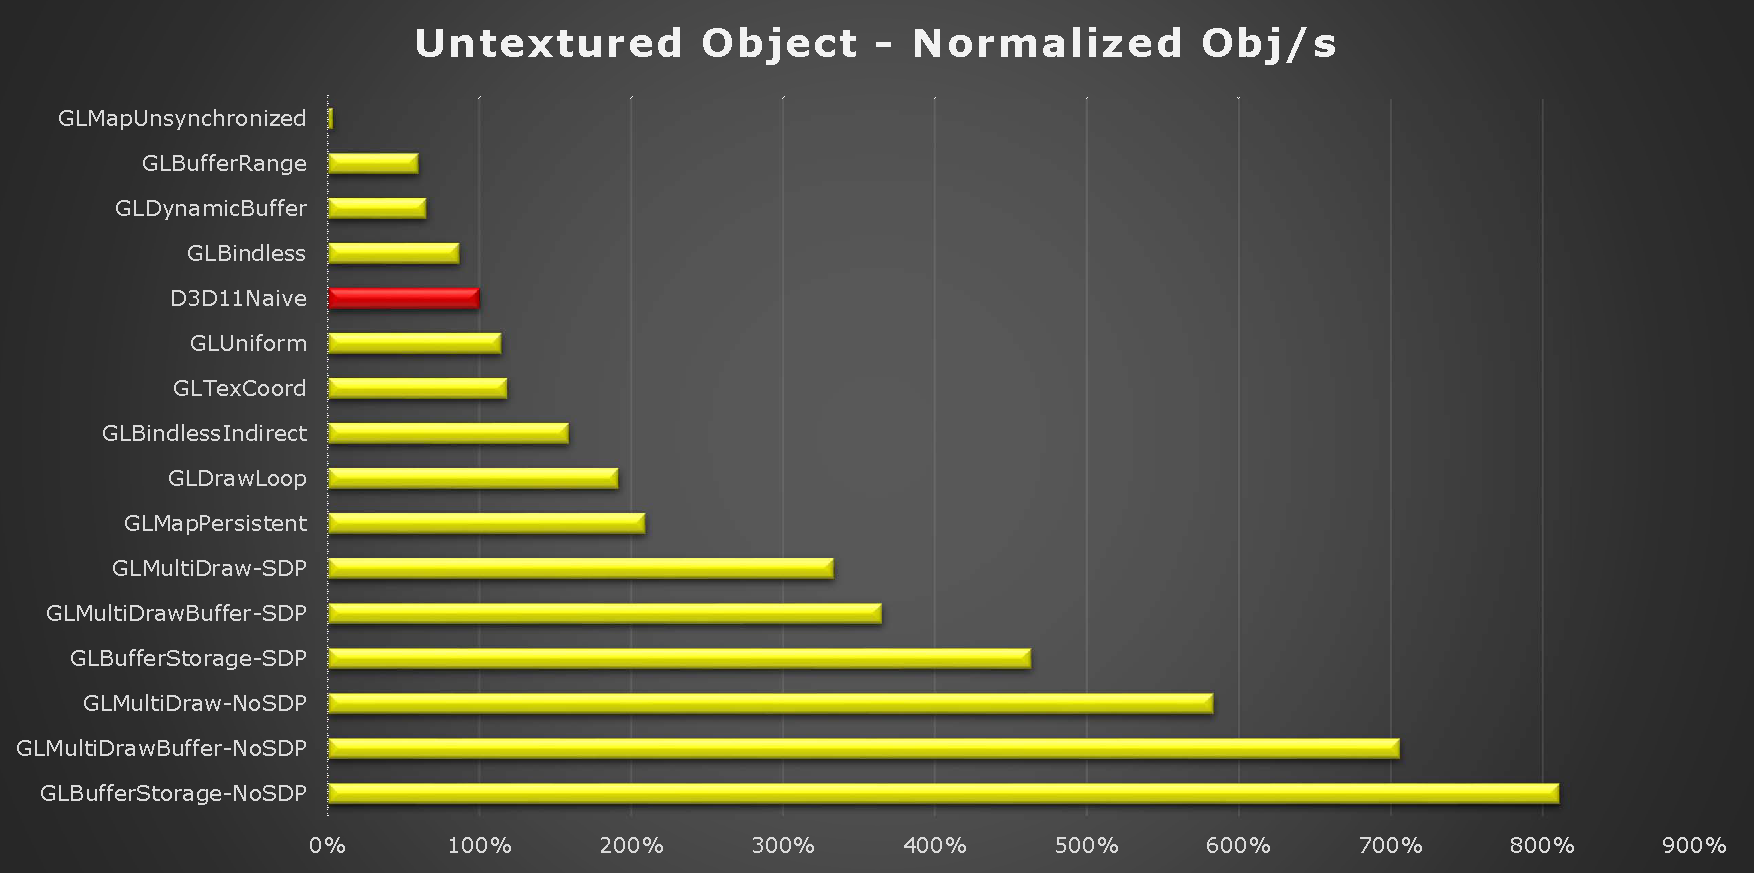
\includegraphics[width=\textwidth]{opengl-spread}
	\caption[Unterschiede in den OpenGL Renderpfaden]{Unterschiede in den OpenGL Renderpfaden \parencite[Seite 98]{Everitt2014}}
	\label{fig:opengl-pfade}
\end{figure}

\paragraph{Multi Draw Indirect} 
\ac{MDI} beschreibt das Ausführen von mehreren Renderanweisungen (Draw-Calls) mit einen \ac{API} Aufruf. Anstatt für jedes Objekt die notwendigen Aufrufparameter des Draw-Calls separat anzugeben, werden die für alle Objekte notwendigen Parameter in einem \textit{OpenGL} Buffer (\textit{Draw Indirect Buffer} oder auch \textit{Command Buffer}) zusammengefasst. Der einzelne indirekte Draw-Call entspricht im wesentlichen nur noch einem Aufruf mit einem Zeiger auf den Inhalt des Command Buffers. Die Parameter können entweder von der CPU aus bestimmt werden oder direkt auf der GPU (z.B. durch View-Frustum Culling auf der GPU). Das Konzept des indirekten Renderns fasst das indexbasierte Rendern und instanziiertes Rendern zusammen\footnote{https://www.opengl.org/wiki/Vertex\_Rendering\#Indirect\_rendering}. Der Command Buffer, in Verbindung mit dem Draw-Call, beschreibt ausschließlich die Gestalt des für alle Objekte gemeinsamen \textit{Vertex} Buffers. Da nun für jedes Objekt kein seperater Draw-Call ausgeführt wird, können auch keine individuellen Daten pro Objekt,zum Beispiel Transformationsmatrizen, an die Shader übergeben werden. Das macht es erforderlich entsprechende Daten gebündelt in einem Array oder \ac{SSBO} dem Shader zu übergeben. Der indizierte Zugriff kann im Shader dann über eingebaute Variablen erfolgen. Dies reduziert zusätzlich den Overhead.

\paragraph{Direct State Access} Ein weiterer Schritt zur Reduzierung des Treiber Overheads ist die \ac{DSA} Erweiterung von \textit{OpenGL} die seit der Version 4.5 zum \textit{Core} Profil von OpenGL zählt \parencite{Akeley2015}. Die unterschiedlichen OpenGL Objekte besitzen meistens einen eigenen internen Zustand. Soll dieser Zustand aktualisiert oder abgefragt werden, müssen bisher die Objekte zuvor über Selektoren gebunden werden. Dies ist oft nicht nur fehleranfällig, sondern sorgt für wenig intuitiven und schwer lesbaren Quelltext. Zusätzlich erhöht es mit zunehmender Szenenkomplexität den \ac{API} Overhead.

Mit \ac{DSA} entfällt das Selektieren von Objekten vor dem Zugriff auf den Zustand. Es werden neue Operationen bereit gestellt, die das entsprechende OpenGL Objekt als Parameter erwarten. So lässt sich der Zustand abfragen und manipulieren, ohne dass das Objekt vorher im globalen Zustand gebunden sein muss. Dies reduziert den Overhead etwas. Im Wesentlichen vereinfacht es die Verwendung der OpenGL Objekte, erlaubt die Kapselung von Funktionalitäten und erleichtert damit die Umsetzung von komponierbaren Bibliotheken \fref{chap:haskell-modern-gl}.

\paragraph{Separate Program Objects} Auch wenn \ac{DSA} erst mit OpenGL 4.5 breiten Einzug ins \textit{Core} Profil genommen hat, fand die Erweiterung |ARB_separate_program_objects| schon mit Version 4.1 ihren Weg in das \textit{Core} Profil \parencite{Akeley2010}. Zuvor mussten die unterschiedlichen Shader Stufen (Vertex, Geoemetry, Fragment usw.) in ein monolithisches Programm übersetzt werden. Mit der Erweiterung können die einzelnen Stufen unabhängig voneinander übersetzt werden. Die Program-Objekte lassen sich dann, unter der Berücksichtungen der Schnittstellen, frei zu einer \textit{Program-Pipeline} zusammensetzen. Zusätzlich führt die Erweiterung \ac{DSA} für die Program-Objekte ein, so dass die Shader-Objekte nicht mehr vor der Uniform-Variablenzuwesung global gebunden werden müssen. Stattdessen können die Zuweisungen direkt mit dem Program-Objekt durchgeführt werden (siehe \fref{sec:haskell-gl-anwendung}).

% ### http://www.g-truc.net/post-0320.html

\section{Vulkan}\label{sec:vulkan}

Vulkan basiert (vormals \textit{glNext}) nicht mehr auf \textit{OpenGL}, sondern wurde im März 2015 als eine neue Grafik-API angekündigt. Noch ist die Spezifikation am entstehen, aber das erklärte Ziel von Vulkan ist die Reduzierung des CPU Overheads, die breitere Ermöglichung von Multi-Threading und die Abschaffung des impliziten OpenGL Context hin zu einer expliziten API. Neben \textit{Vulkan} wurde \textit{SPIR-V} als eine neue Shader \ac{IL} bzw. Zwischensprache vorgestellt. SPIR-V soll neue Freiräume schaffen eigene Shader-Sprachen sowie Analsyse- und Debuggingtools zu entwickeln \parencite{Olson2015}.

Die Gründe für einen harten Schnitt in der \ac{API} sind auf zwei Seiten zu suchen. Zum einen ist für den API-Anwender die OpenGL-API, wie bereits erwähnt, voller Fallstricke und das Hardware-Abstraktions-Modell gilt als veraltet. Auf der anderen Seite stellen die  OpenGL Treiber aller Hersteller aus softwaretechnischer Sicht ein großes Problem dar. Die Treiberimplementierungen verwenden viele Spezialregeln, die zur Laufzeit einer Grafikanwendung angewendet werden. Entweder um bekannte Fehler in der Anwendung der API abzufangen oder potenziell langsame Pfade in schnellere Pfade zu übersetzen \parencite{gamedevnet:glnext}. Das das führt dazu, dass die Wartung der Treiber für die Hersteller aufwändig geworden ist.

Auf Grund der bisher noch fehlenden Spezifikation von \textit{Vulkan}, lässt sich die neue API noch nicht beurteilen. Doch wurde offiziel, nach der Einstellung von \textit{AMD Mantle}, bekannt gegeben, dass \textit{AMD Mantle} die technologische Basis für die \textit{Vulkan} \ac{API} stellen soll\footnote{http://community.amd.com/community/amd-blogs/amd-gaming/blog/2015/03/03/one-of-mantles-futures-vulkan}. {AMD Mantle} verfolgte das gleiche Ziel wie \textit{Vulkan}. \textit{AMD Mantle} bildete eine Teilfunktionalität aktueller Grafik-\acp{API} ab und entsprach einer auf den oben genannten \ac{AZDO} Konzepten konzentrierten \ac{API}.

\begin{figure*}
\centering
	
\includegraphics[height=2cm]{Vulkan_Mar15}
	
\includegraphics[height=2cm]{SPIR_Nov14}
\end{figure*}


